\section{Privacy Protection against Real-World Apps}
\label{sec:protecting_up}

%With their vast array of apps and services, Android devices often require users to grant permissions for accessing various resources and functionalities. While these permissions are necessary for delivering app features and services, they can also threaten user privacy when sensitive data is shared with third-party apps. \framework{} is designed to spoof the user data fed into apps that protect user privacy by preventing the sharing of sensitive user data with third-party apps while enabling users to enjoy app features without compromising essential functionalities that rely on those permissions.

%The Android permission framework controls access to sensitive resources and user data. Apps declare the permissions they require, such as accessing contacts, location, or device sensors, during the installation process. Users are then presented with the option to grant or deny these permissions. While this mechanism ensures that apps have the necessary access to provide desired features, it also raises concerns about the privacy implications of sharing personal data with potentially untrusted apps.

% \framework{} addresses these privacy concerns by allowing users to manipulate and spoof the user data presented to apps. With \framework{}, users gain greater control over sharing their personal information, ensuring that sensitive data remains protected and inaccessible to third-party apps. By selectively modifying user data, \framework{} enables users to enjoy app features without compromising their privacy or granting unnecessary access to personal data.

%this ensures that sensitive information remains safeguarded, reducing the risks associated with unauthorized data access and potential privacy violations.

%The findings shed light on the benefits of using \framework{} to enhance user privacy and balance app functionality and data protection. Ultimately, \framework{} offers a novel approach to safeguarding user privacy in the Android ecosystem, allowing users to enjoy apps while retaining control over their personal information.

In Figure~\ref{fig:intro-case-study-uber}, we showed how \framework can be
effectively used to protect user privacy while they are using Uber.  In this
section, we use three more real-world Android apps to showcase privacy
advantages of \framework.

\subsection{com.katana.facebook (v404.0.0.35.70)}
\label{sec:fb_case_study}
% Facebook claims that while ads may seem highly specific, as if the app is eavesdropping on conversations through the microphone, they deny such practices and state that audio permissions are only used for in-app features. However, experimental evidence paints a different picture of how Facebook utilizes permissions in the background.

% For the purpose of conducting experiments, the 
% The Facebook app was granted all the requested permissions.
%mentioned in the Manifest file. Using \framework{}, these permissions were manipulated. 
During the experiment, while scrolling through posts in the Facebook app's
\textit{Home} activity and without engaging any other app features,
\framework's \textit{Resource Access Log Reporter} recorded instances of the
Facebook app accessing audio permission as shown in
Figure~\ref{fig:case-study-facebook}(a). On further investigation, we found
that the Facebook app was using \texttt{MediaRecorder} to access the device
microphone. Moreover, the Android's privacy indicator~\cite{andPrivacyIndicator}
(green dot), which indicates active use of the device microphone, did not appear
when \framework{} logged the use of audio permission. We found this surprising.

We were able to repeat this behavior with a custom mobile app i.e. we used
\texttt{MediaRecorder} API to successfully record audio
% without user knowledge; we were successful in recording audio from the device
% microphone 
while Android's privacy indicator did not show up. We believe it is a bug in
Android's privacy indicator implementation. We have reported this to Android and
plan to open source this custom app responsibly.

Hence, \framework{} was able to detect microphone usage that was not indicated
by Android. Moreover, \framework{} successfully spoofed audio data requested
by the Facebook app. 
% We cannot ascertain how Facebook utilizes the recorded
% audio files recorded by the app, but it is clear that they capture audio data
% from the device microphone that is not indicated by the Android to the user. 
% Therefore, \framework can help users
% to detect such usage by the apps and can protect privacy by spoofing the user
% data.

Similar to the unexpected microphone access, \framework{}
% 's \textit{Resource Access Log Reporter} 
also logged instances of calendar data access by the Facebook app while
searching for nearby events. The app reads user's calendar events to display their
availability when the user is viewing nearby events.  
% As an intelligent spoofing technique, 
Users can configure \framework to manipulate calendar data in a way that allows
the Facebook app to receive information about their availability without
compromising sensitive details about individual events. This involves spoofing
fields like event name and location. 
% within the \texttt{CalendarContract.EventsColumns} class, excluding fields that define the
% event's duration.  
\framework could spoof the app's request for calendar data by providing a list
of manipulated events.

\begin{figure}[t]
    \centering
    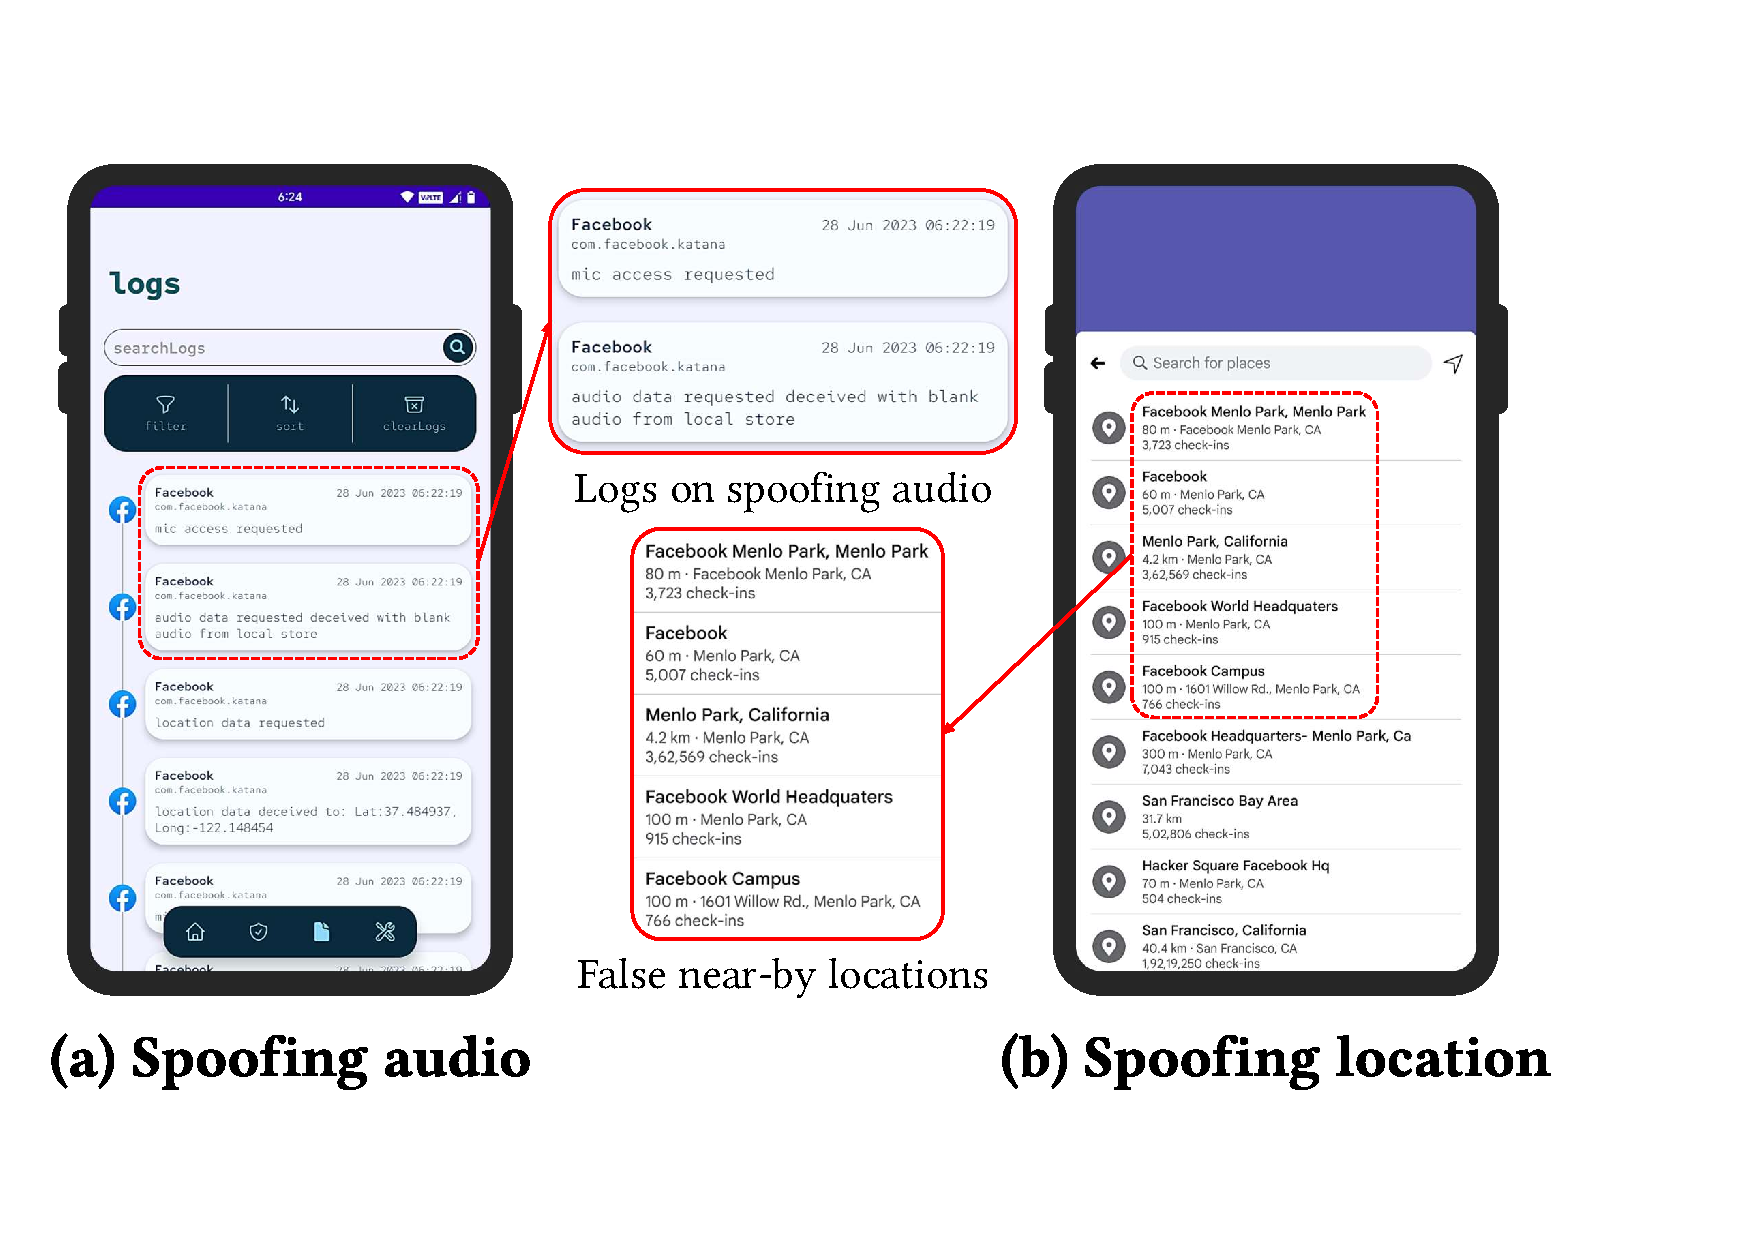
\includegraphics[width=\linewidth]{Figures/Case Studies/facebook_screenshots.pdf}
    \caption{Screenshots demonstrating deceiving location and audio data using \framework{} for the Facebook app.}
    \label{fig:case-study-facebook}
\end{figure}

% \begin{figure}[t]
% \centering
% \begin{subfigure}{0.48\linewidth}
%     \centering
%     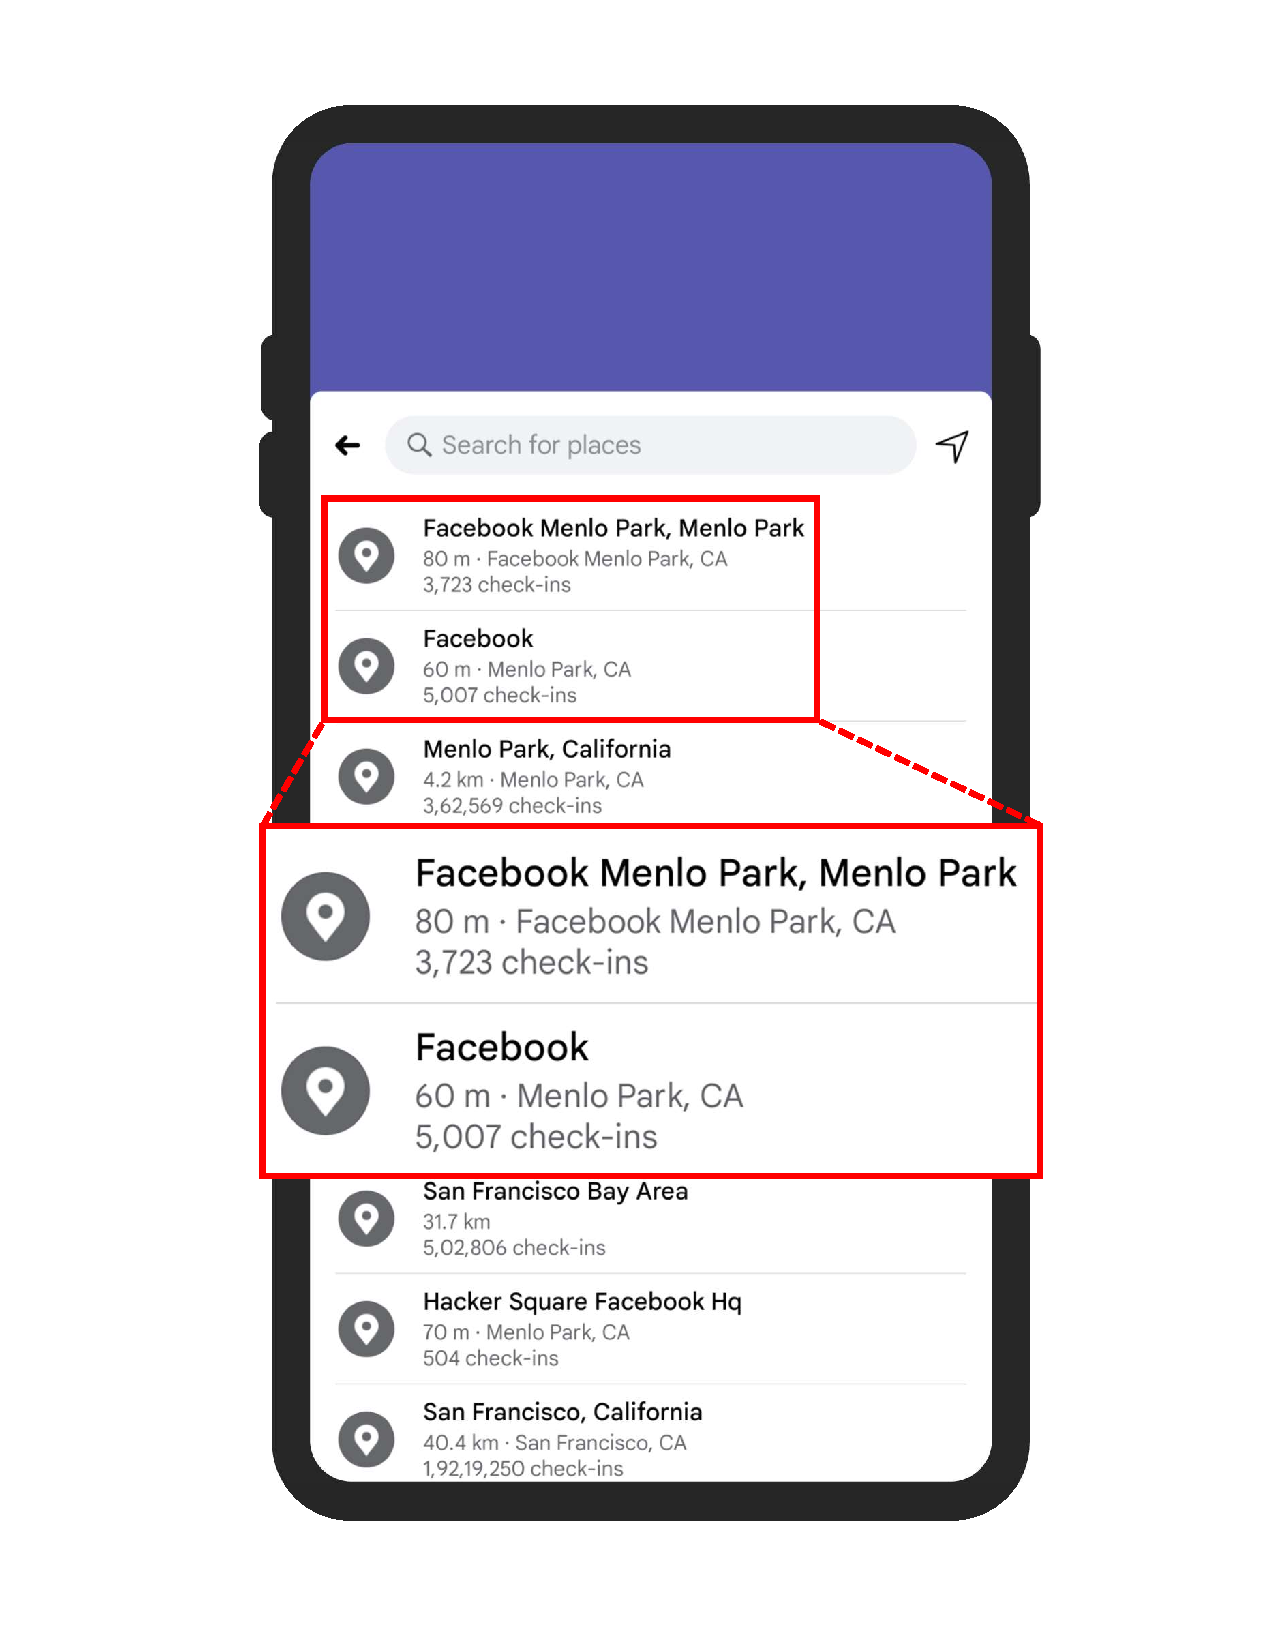
\includegraphics[width=0.8\linewidth]{figures/case_studies/fb_after_deceiving.pdf}
%     \caption{With \framework{} (False nearby locations (Facebook's HQ) presented to user)}
%     \label{fig:case-study-facebook_w_frmwrk}
% \end{subfigure}
% \begin{subfigure}{0.48\linewidth}
%     \centering
%     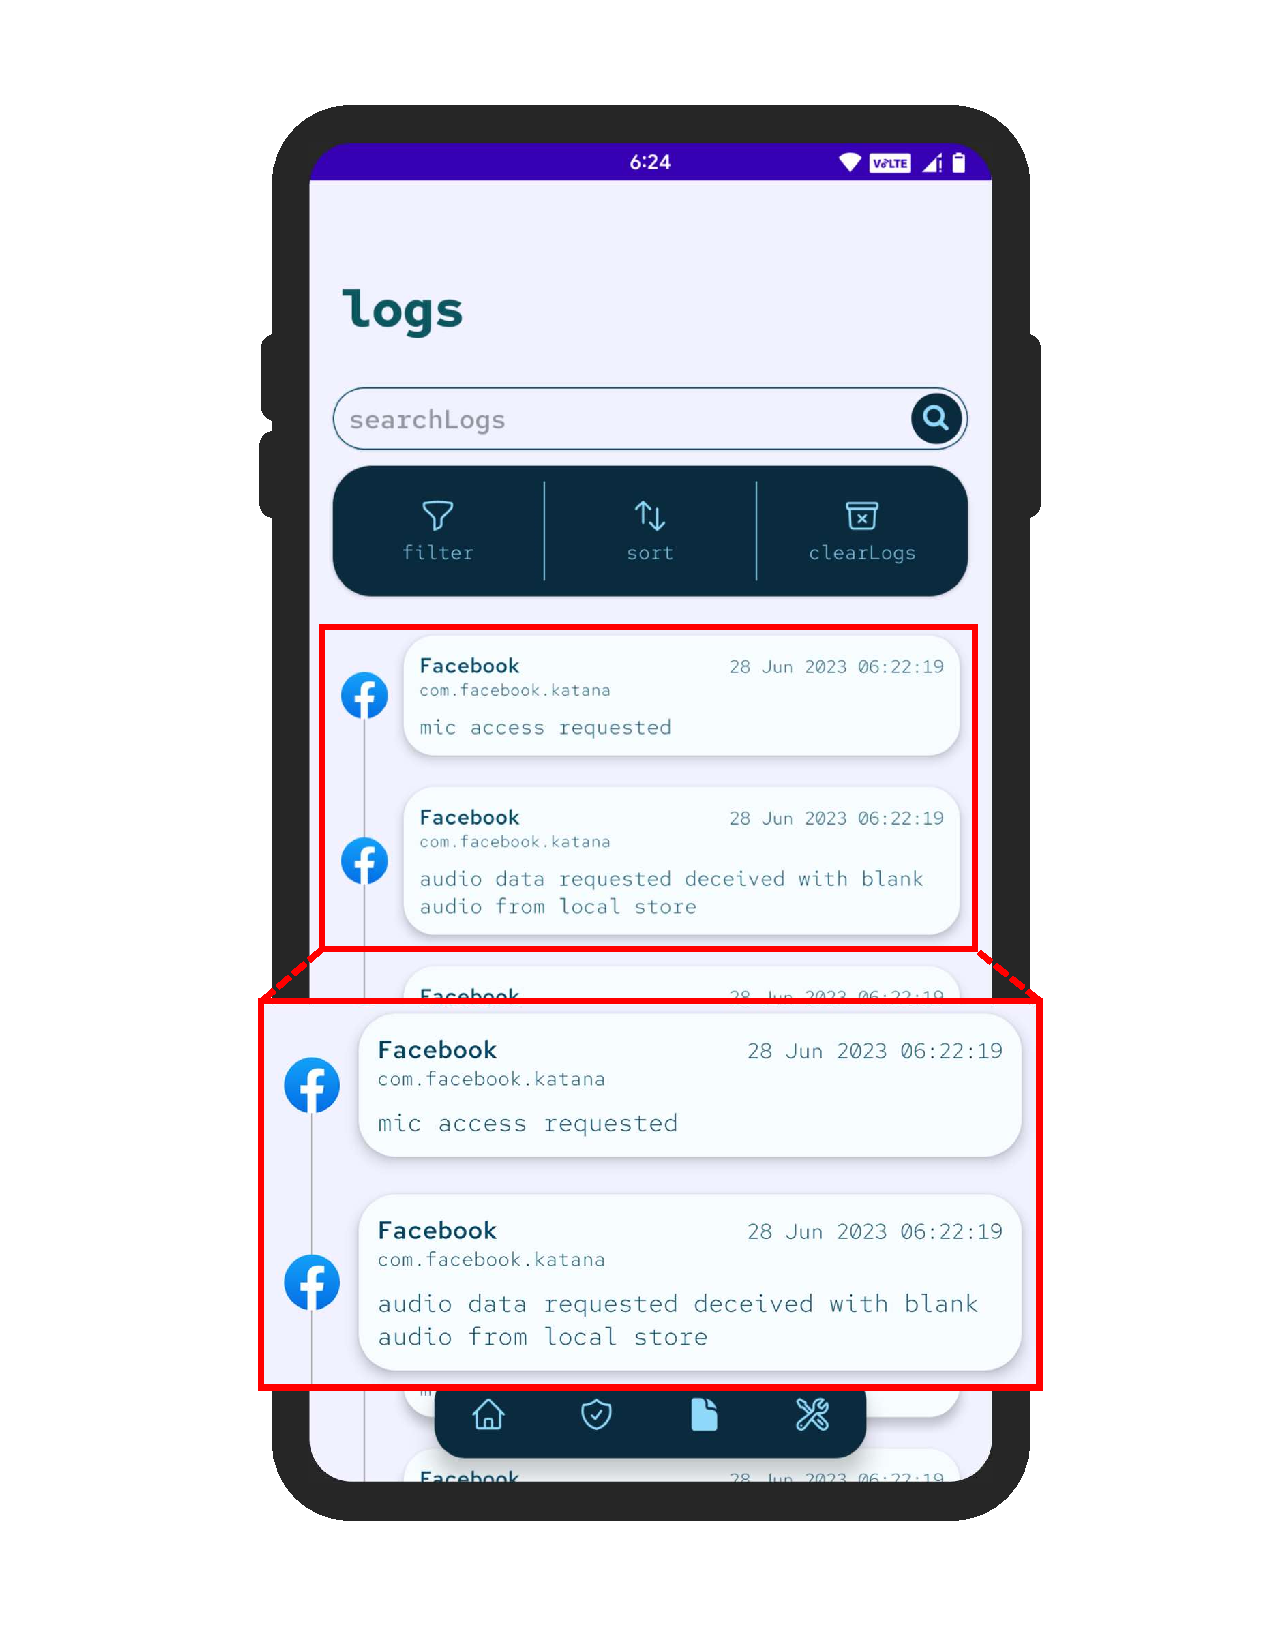
\includegraphics[width=0.8\linewidth]{figures/case_studies/fb_mic_access_log.pdf}
%     \caption{Without \framework{} (True nearby locations presented to user)}
%     \label{fig:case-study-facebook_wo_frmwrk}
% \end{subfigure}
% \caption{Screenshots of \textit{Facebook} while tagging location for post creation (\textit{Facebook} presenting nearby locations by accessing GPS location of the device)}
% \label{fig:case-study-facebook}
% \end{figure}

% In addition to Facebook's deceptive activities, 
% Notably, the feature that enables users to add location to their stories on the
% app requests live GPS location data to provide a list of nearby places for easy
% location tagging. Similarly, 
Nearby events were listed using user's location
data. As shown in Figure~\ref{fig:case-study-facebook}(b), we could
effectively spoof the fine-grained GPS location data with a nearby location
ensuring that the reported nearby places and events were same without
compromising user's exact location. 
% associated with the
% manipulated (spoofed) location rather than the original one, 
% This is shown in 
% To summarize, \framework successfully
% spoofed various permissions requested by the app, including access to accounts,
% audio, calendar, camera, clipboard, and location, among others. 

% \subsection{com.ubercab (v4.462.10000)}
% \label{sec:ub_case_study}
% If a user, concerned about potential privacy breaches, denies GPS access to the
% Uber app, the app loses its ability to find the closest cab. Conversely, if the
% user grants GPS access, the app successfully locates the nearest cab.
% % Unfortunately, this also means that the user's live location is shared with Uber
% % servers, compromising privacy. We initially searched for cabs using Uber by
% % providing our GPS location data, as shown in
% % Figure~\hyperref[fig:intro-case-study-uber]{1a}. This fulfilled the user's
% % requirement but at the cost of compromising the GPS data. 
% % The blue circle represents our GPS location, while the black pin indicates the desired pickup location. However, once an app obtains permission to access the GPS location, it retains that access until the user manually revokes it. Consequently, Uber continues to acquire GPS data from the device whenever the user utilizes the app (if "Allow only while using the app" is selected during permission granting). 
% % To mitigate this situation, users can navigate to their device settings and revoke the permissions temporarily when they do not wish the app to access their location. Nevertheless, this approach may not work with every app, as many apps cease functioning entirely or partially if the requested permissions are not granted. 
% % This is where \framework{} becomes invaluable, allowing users to determine which data they share with apps by spoofing the information provided in response to permission requests.
% % To put this into action, we accessed the pre-installed and activated \framework{} module on our device and selected Uber's location permission to spoof, as depicted in Figure X. Next, we utilized \framework{}'s "Deceits" section to define the desired latitude and longitude for the new location we wanted the target app to receive when requesting location data. Now, when Uber restarts and requests the device's GPS location, it receives the spoofed location instead of the actual one. This way, users can protect their privacy and enjoy app features without compromising their personal information.
% % However, instead of revoking the location permission in the app, utilizing
% As shown in Figure~\ref{fig:intro-case-study-uber}(b), \framework with the Uber
% app kept the features of the Uber app stable and we were successfully able to
% find the nearest cab without compromising the original GPS data as shown in
% Figure~\hyperref[fig:intro-case-study-uber]{1b}.

% The information regarding Uber's access to GPS location is logged in the \framework{} logs, as shown in Figure X. Users can refer to these logs to investigate apps and determine whether the resource data access was for legitimate app features or potentially malicious activities.

\subsection{com.snapchat.android (v12.24.0.34)}
\label{sec:sc_case_study}
%Since January 2014, Snapchat has been plagued by a series of security breaches, resulting in the compromise of private information belonging to millions of users. These breaches have disproportionately impacted innocent users who have little to no control over their personal data stored on these app servers. However, \framework{} introduces an additional layer of security, empowering users with control over the data they transmit to servers and store in databases.

\begin{figure}[t]
    \centering
    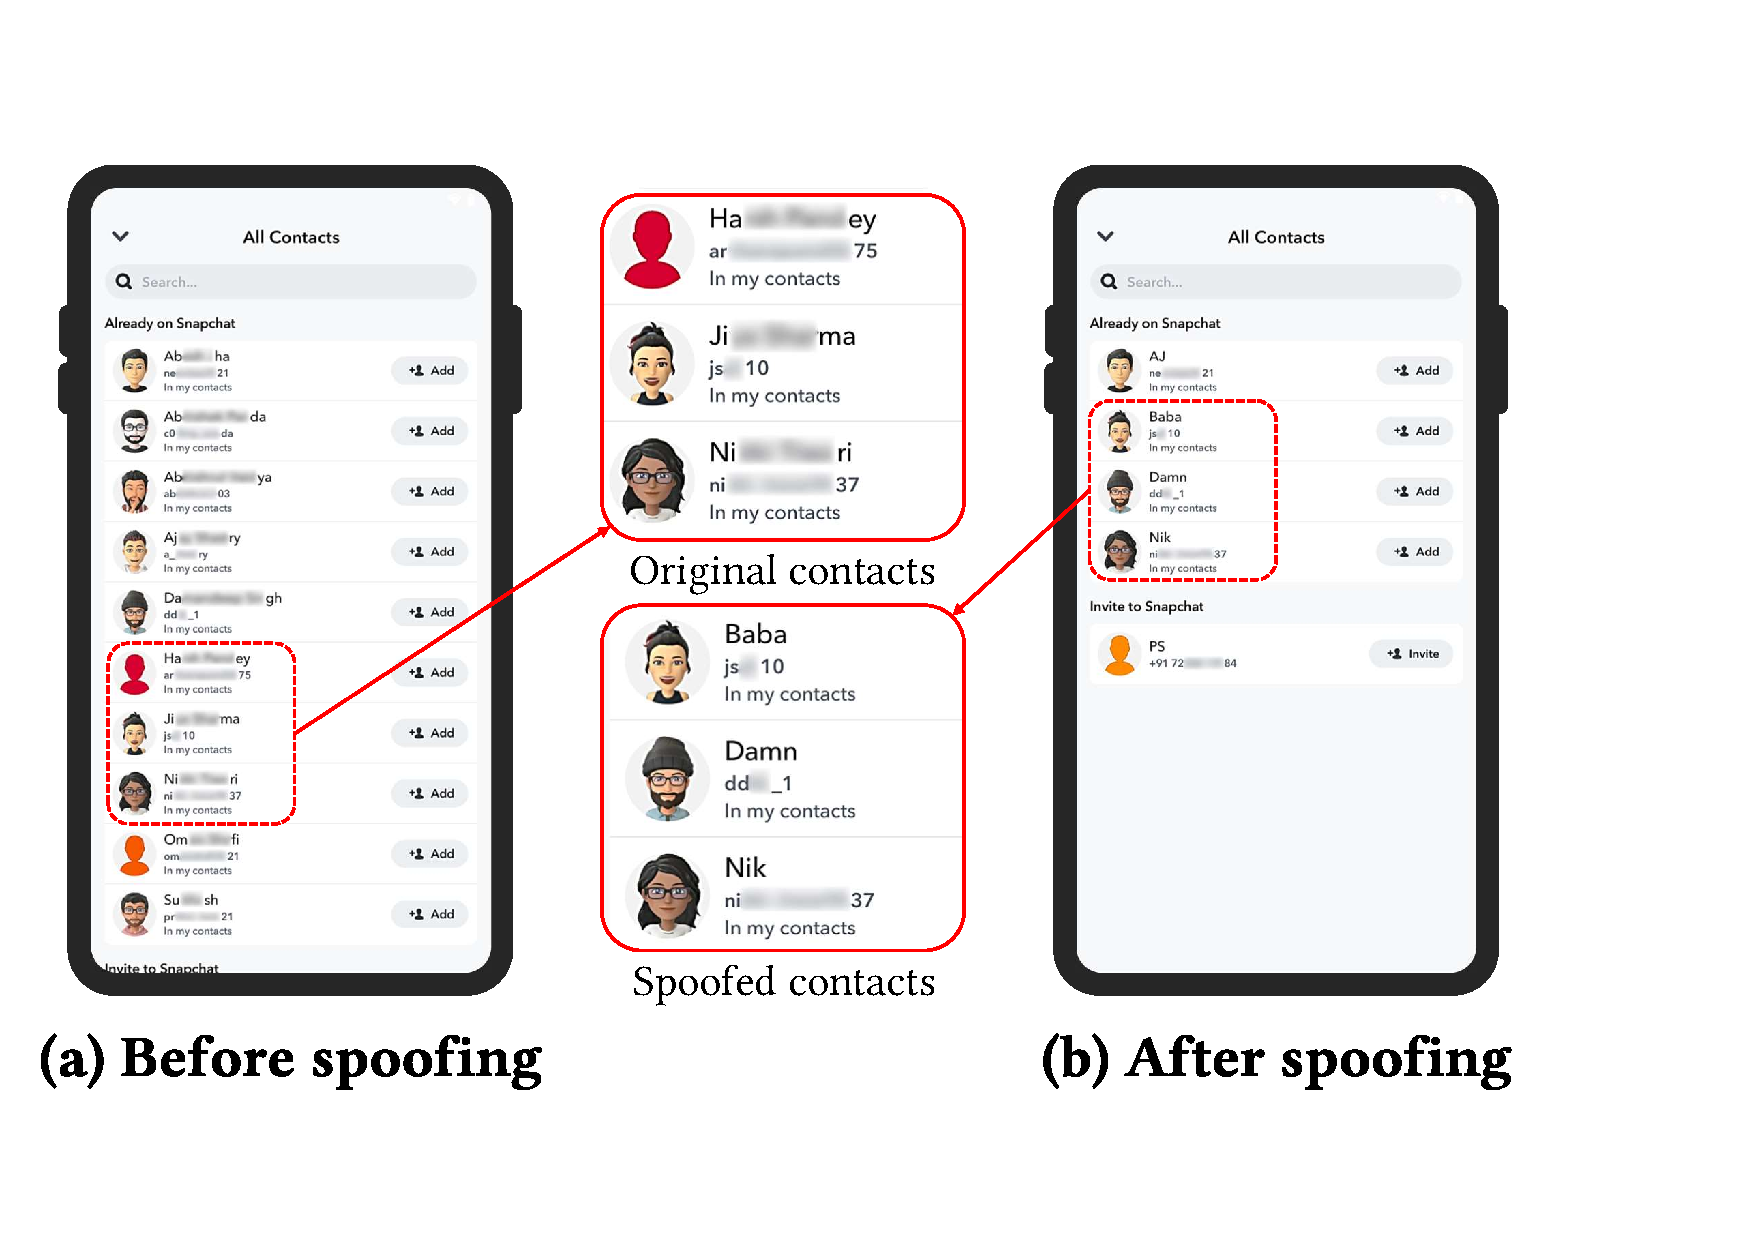
\includegraphics[width=\linewidth]{Figures/Case Studies/snapchat_screenshots.pdf}
    \caption{Screenshots demonstrating how user can share spoofed contacts using WhiteLie with Snapchat.}
    \label{fig:case-study-snapchat}
\end{figure}

% \begin{figure}[t]
% \centering
% \begin{subfigure}{0.48\linewidth}
%     \centering
%     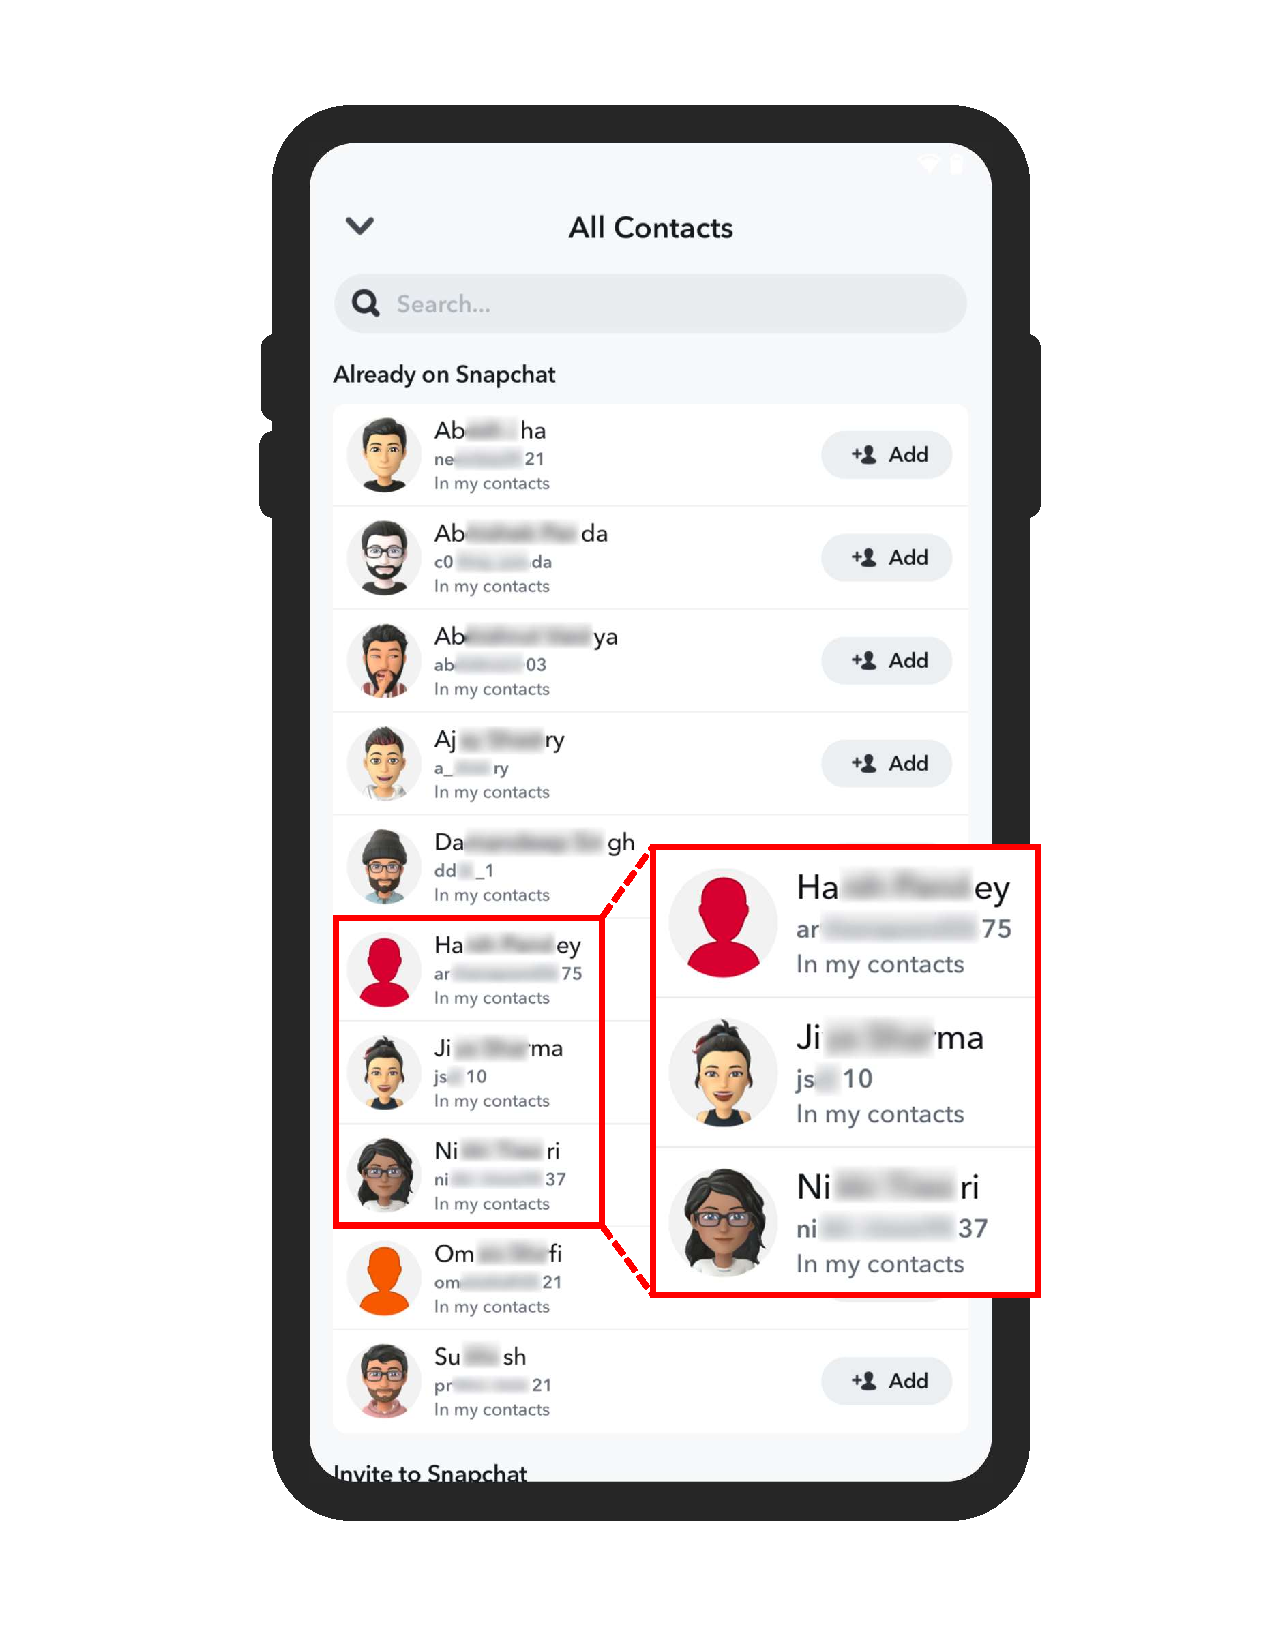
\includegraphics[width=0.8\linewidth]{figures/case_studies/snapchat_before_deceiving.pdf}
%     \caption{Without \framework{} (All contacts with original names are presented to user)}
%     \label{fig:case-study-snapchat_wo_frmwrk}
% \end{subfigure}
% \begin{subfigure}{0.48\linewidth}
%     \centering
%     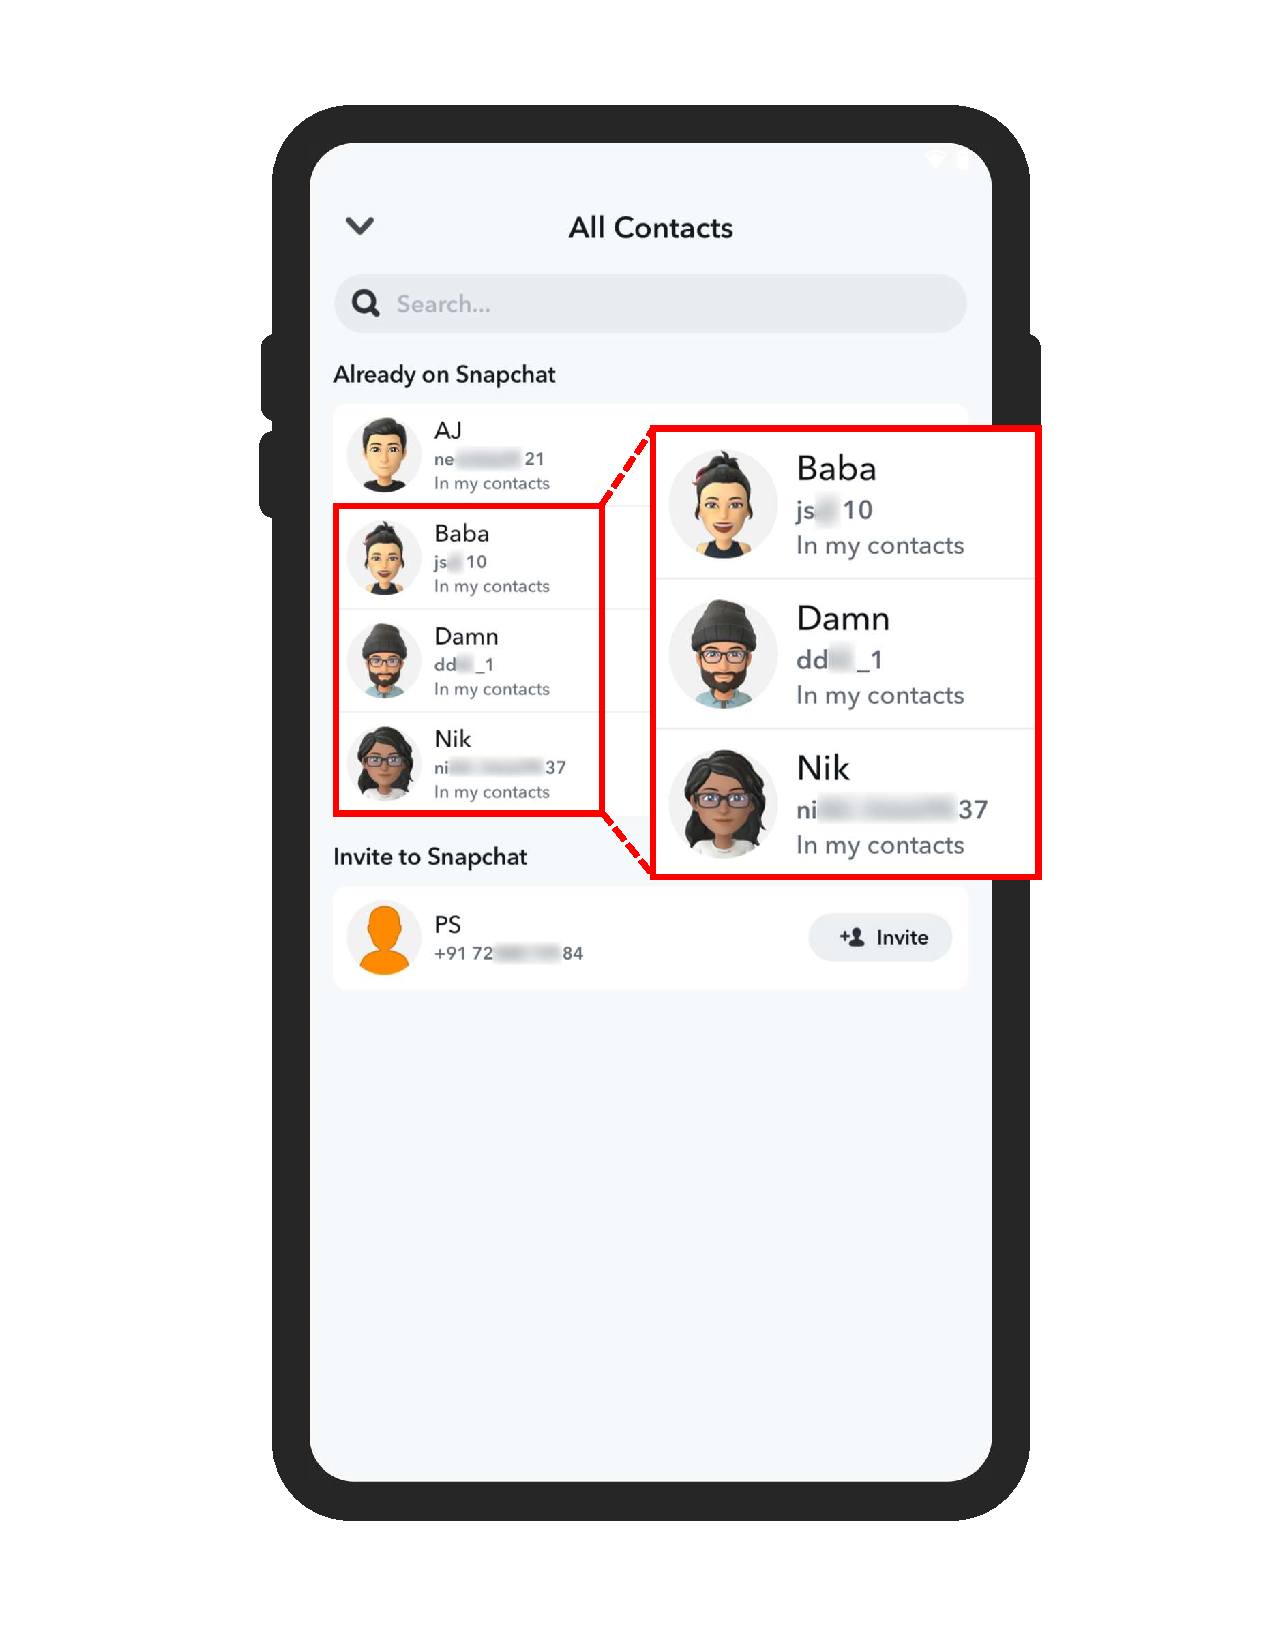
\includegraphics[width=0.8\linewidth]{figures/case_studies/snapchat_after_deceiving.pdf}
%     \caption{With \framework{} (Contacts as defined in the \textit{Deceit} policy of \framework{})}
%     \label{fig:case-study-snapchat_w_frmwrk}
% \end{subfigure}
% \caption{Screenshots of \textit{Snapchat} while finding new friends (\textit{Snapchat} presents user accounts by accessing Contacts of the device)}
% \label{fig:case-study-snapchat}
% \end{figure}

Snapchat has a feature called 
% attracts users with a range of appealing features, leading them to make privacy concessions in exchange. One such feature is 
\textit{Snap Map}, which utilizes the device's GPS and other sensors to
display user avatars on a map, showcasing real-time physical activities. 
% While
% this fosters better social connectivity among friends, it also exposes users'
% private location, essentially allowing unauthorized surveillance without
% their knowledge or consent. 
While Snapchat does provide \textit{Ghost Mode} as
an option to refrain from sharing location and sensor data, it sacrifices
\textit{SnapMap} features that rely on this information. Furthermore,
\textit{Ghost Mode} does not guarantee that the app is not accessing the data. 

%In contrast, \framework{} presents a far superior alternative, spoofing the app with manipulated data to make it believe that the provided information is genuine. This enables users to enjoy the app's features while safeguarding the privacy of their data.

\framework successfully spoofed device's GPS location and
\texttt{READ\_CONTACTS} by utilizing a list of contacts specified in
\framework's \textit{Deceit} section as shown in Figure
\ref{fig:case-study-snapchat}(b). Users can thus limit the information 
they want to share with Snapchat and still use Snap Map feature.

\subsection{com.truecaller (v12.54.7)}
\label{sec:tc_case_study}
Truecaller provides sender information about incoming text messages to highlight
known spammers. With Truecaller, users can ignore spam messages. But to use
this feature, users have to give permission to the app to read all their
messages. 
% However, this convenience comes at a price: users must share their private data
% with Truecaller to benefit from these call and message insights. During our
% examination of Truecaller using 
We used \framework to successfully spoof message content while retaining the phone 
number from which the message was received.
%  user data
% such as messages, contacts, call logs, and locations that Truecaller requested.
This way users can retain control over the privacy of their messages 
while still identifying whether senders are known spammers as shown in
Figure~\ref{fig:case-study-truecaller}(b).

\begin{figure}[t]\centering
    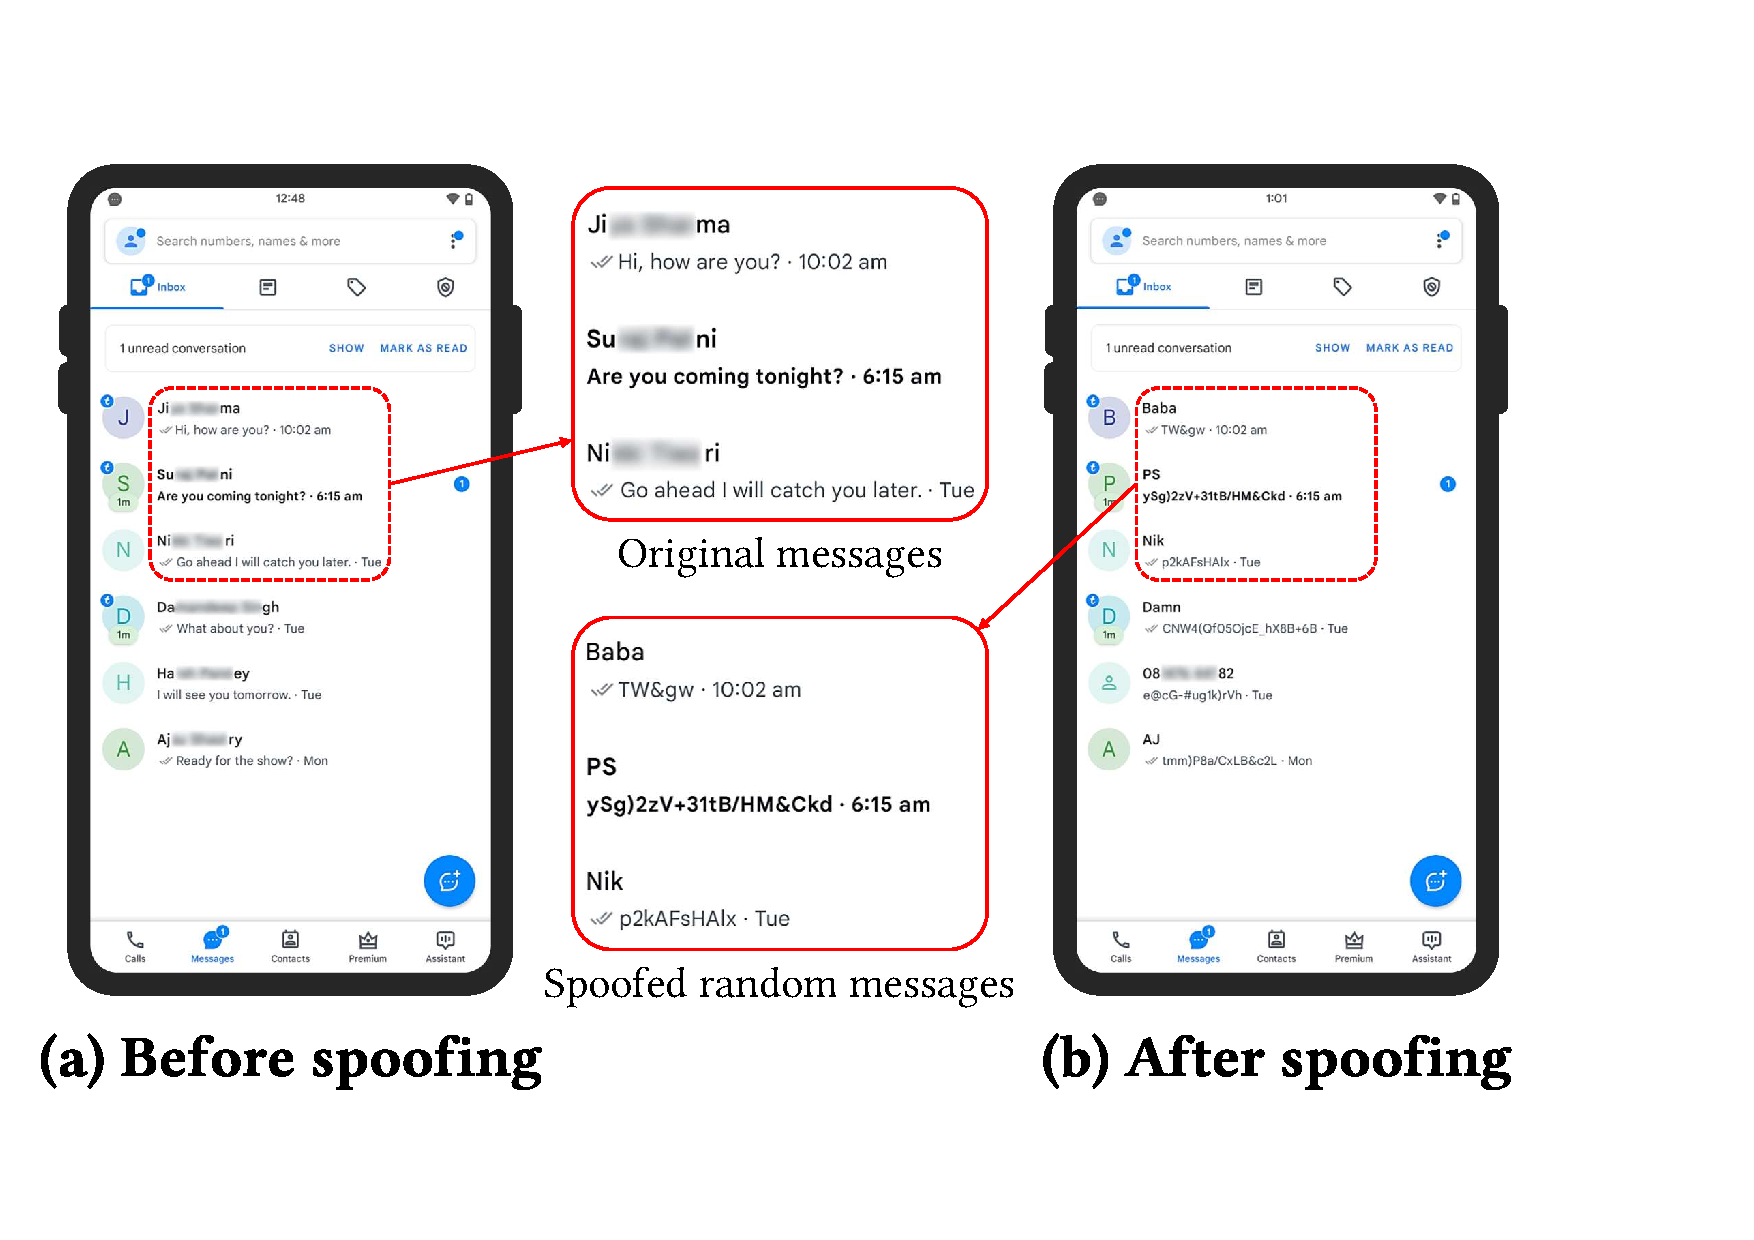
\includegraphics[width=\linewidth]{Figures/Case Studies/truecaller_screenshots.pdf}
    \caption{Screenshots demonstrating how a user can share spoofed SMS using WhiteLie with Truecaller app.}
    \label{fig:case-study-truecaller}
\end{figure}

\textit{Overall, this section shows that \framework empowers users to fully use
the app features while controlling the information that they share with the
apps.}

% \begin{figure}[t]
% \centering
% \begin{subfigure}{0.48\linewidth}
%     \centering
%     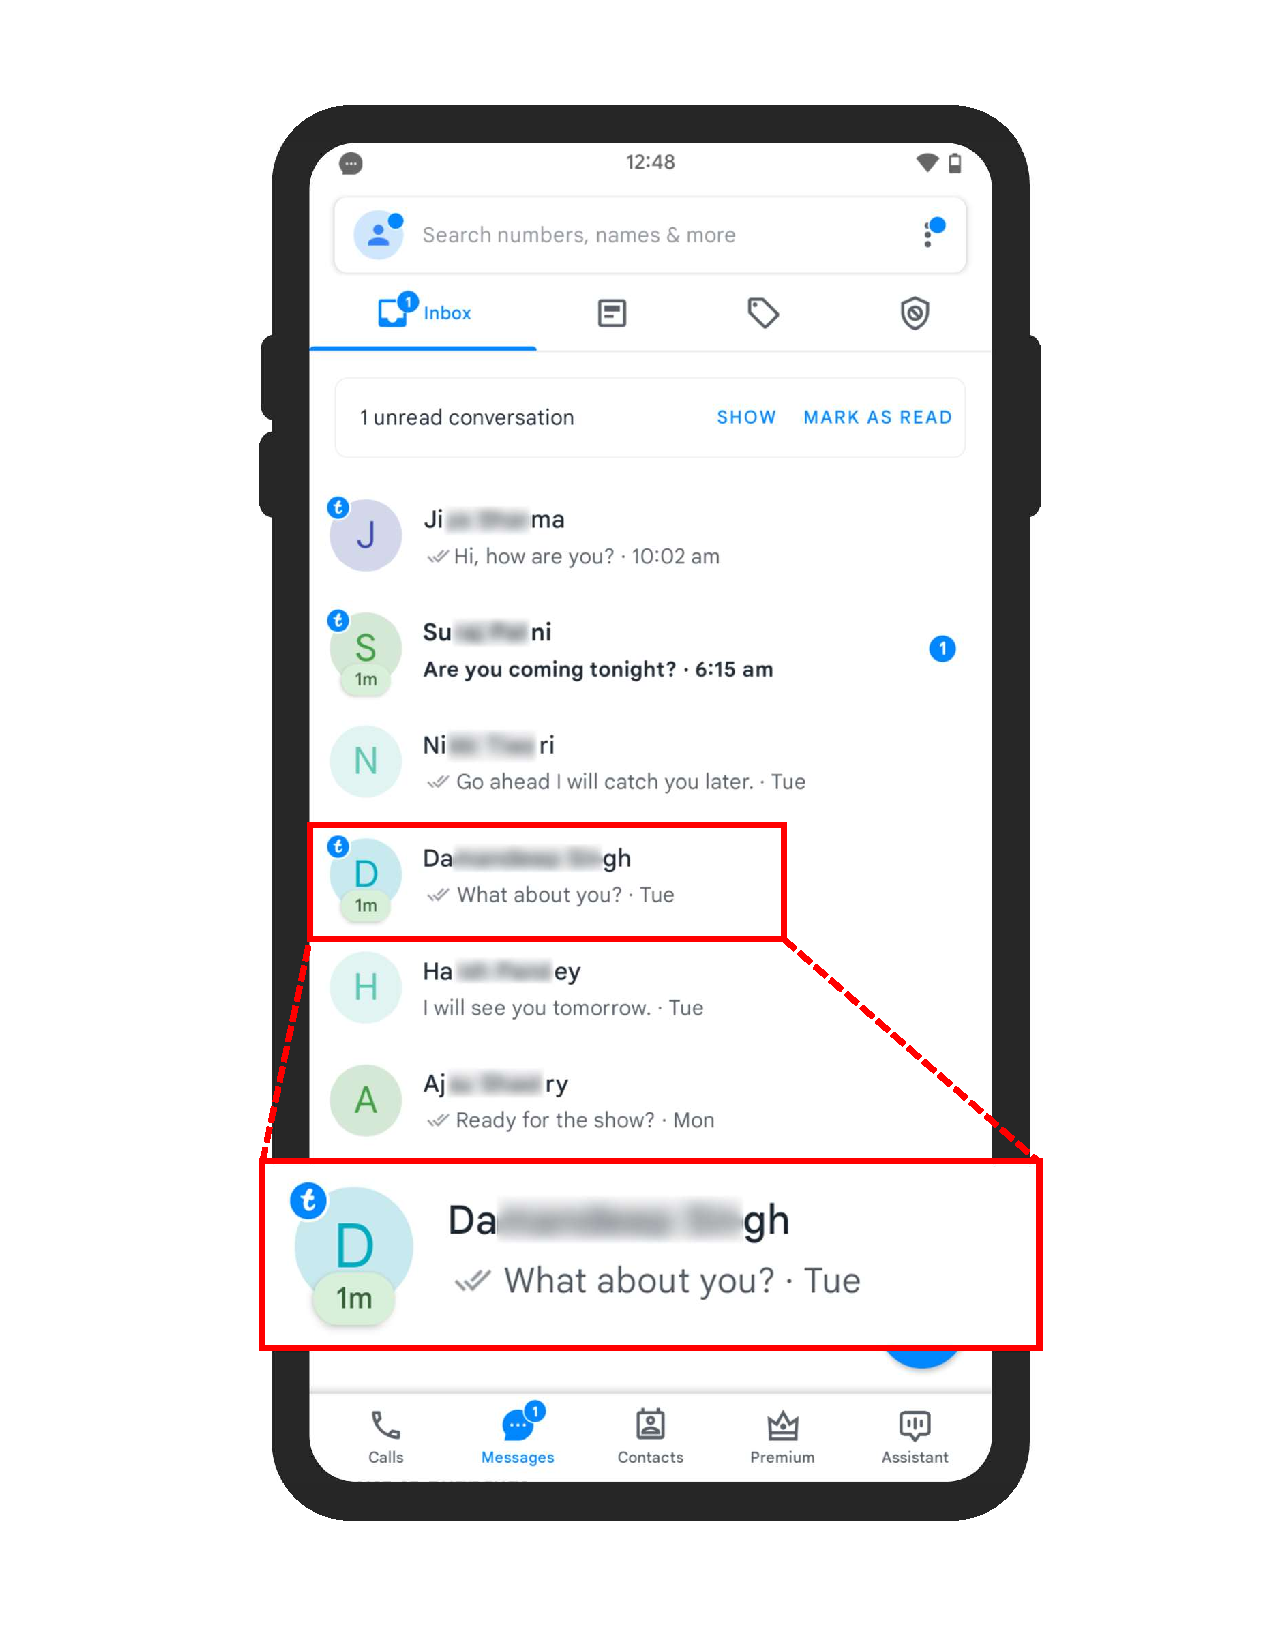
\includegraphics[width=0.8\linewidth]{figures/case_studies/truecaller_before_deceiving.pdf}
%     \caption{Without \framework{} (All contacts with original names are presented to user)}
%     \label{fig:case-study-snapchat_wo_frmwrk}
% \end{subfigure}
% \begin{subfigure}{0.48\linewidth}
%     \centering
%     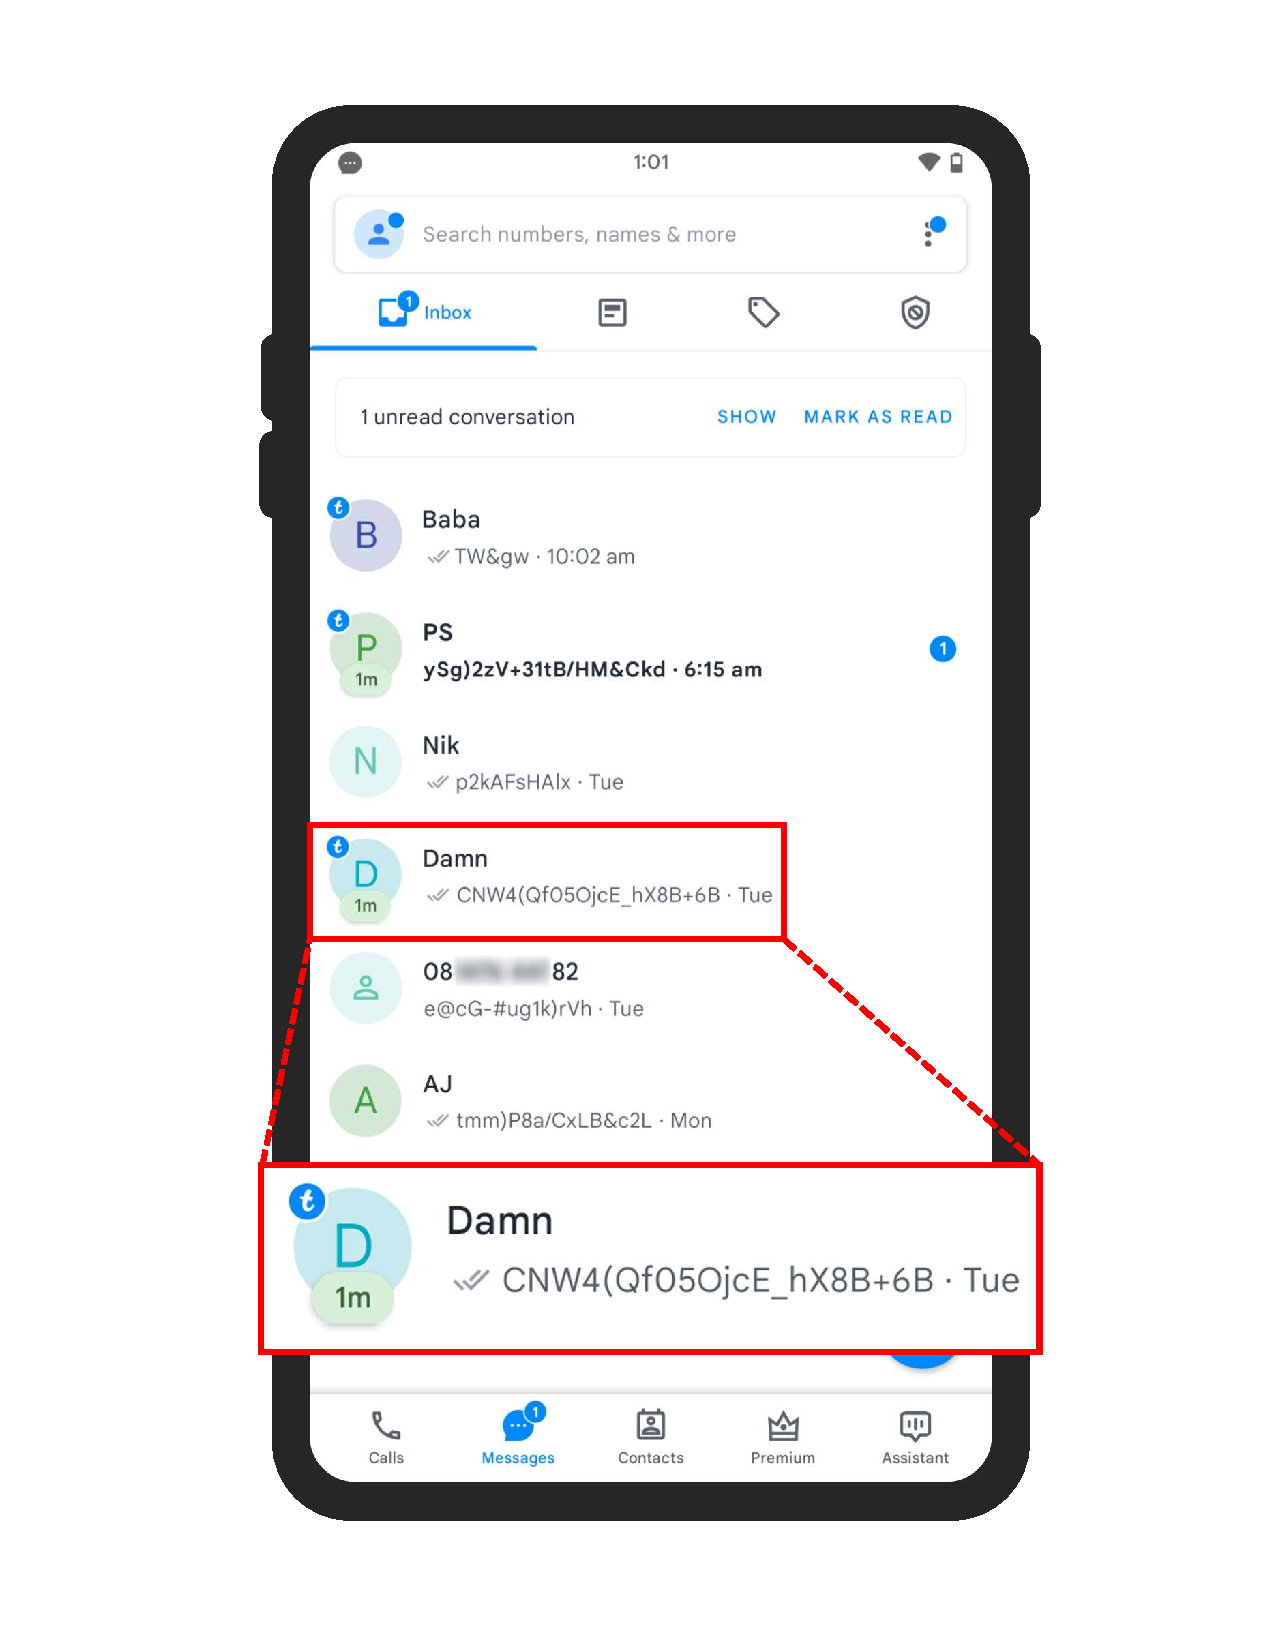
\includegraphics[width=0.8\linewidth]{figures/case_studies/truecaller_after_deceiving.pdf}
%     \caption{With \framework{} (Contacts as defined in the \textit{Deceit} policy of \framework{})}
%     \label{fig:case-study-snapchat_w_frmwrk}
% \end{subfigure}
% \caption{Screenshots of \textit{Snapchat} while finding new friends (\textit{Snapchat} presents user accounts by accessing Contacts of the device)}
% \label{fig:case-study-snapchat}
% \end{figure}

%Truecaller claims to securely store the data shared by users in their database. Nevertheless, allegations have been raised against Truecaller, accusing them of selling users' private information stored in their database. Investigations are currently underway to address these concerns.

%To address these privacy concerns and give end-users control over their shared data, we introduce \framework{}. With \framework{}, end-users can take charge and manipulate the resource data, including contacts, call logs, and messages, using the \textit{Policy Configurator}. 

%\subsection{in.hyiitd.pdp}
%We developed an in-house application called \textit{user data Presenter (PDP)} that requests runtime permissions from the user. However, if the user denies these requests, PDP restricts their access to the application. Once granted permission, PDP retrieves user data from the Android OS and displays it on the screen. Additionally, it stores this data on a remote server using \textit{Google Firebase}, replicating the behavior of typical Android apps. This demonstration emphasizes the ease with which apps can collect sensitive user information from devices and transmit it to remote servers, all without the user's knowledge or any limitations imposed by the Android OS.

%\begin{figure}[t]
%\centering
%\begin{subfigure}{0.48\linewidth}
%    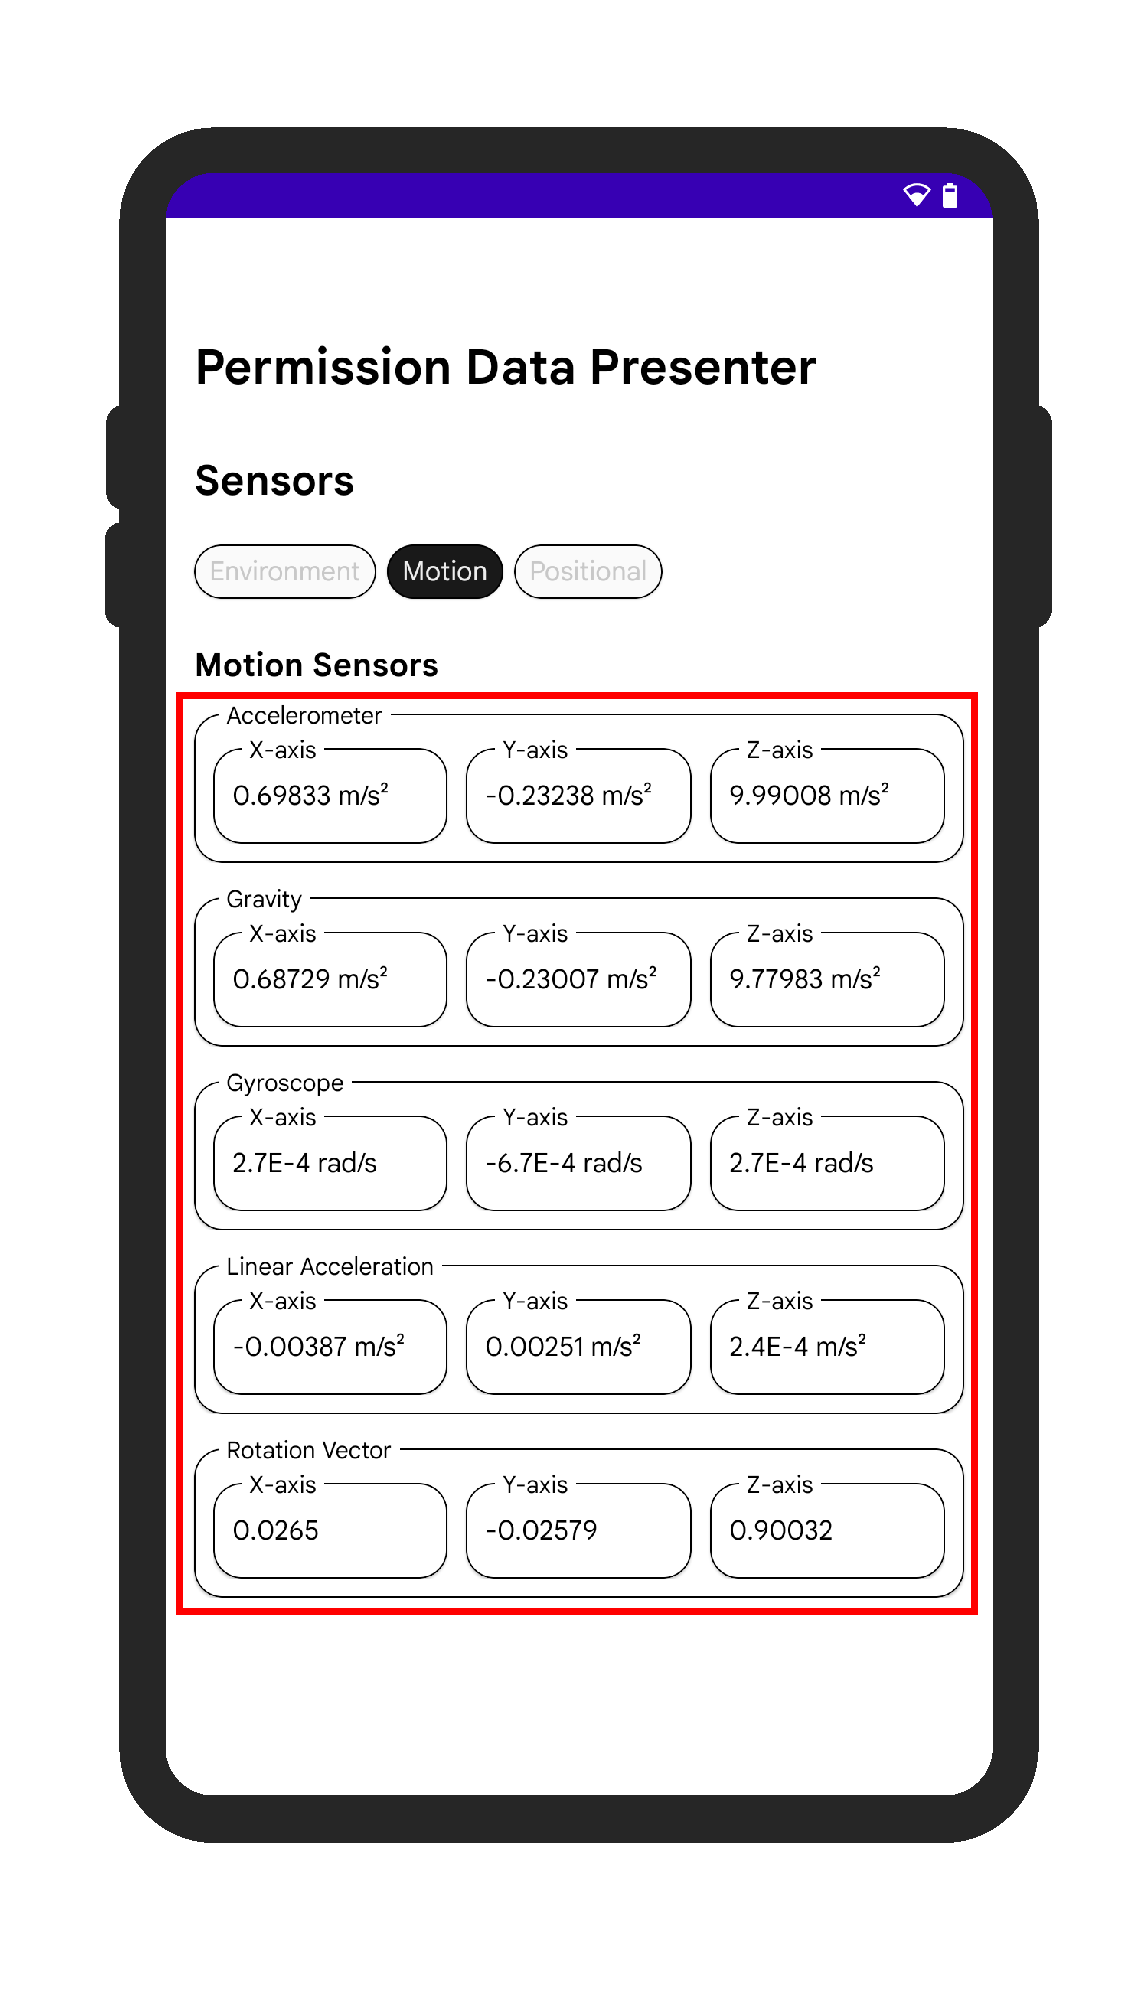
\includegraphics[width=\linewidth]{figures/case_studies/pdp_before_deceiving.pdf}
%    \caption{\centering Without \framework{} (True sensor readings)}
 %   \label{fig:case_study_pdp_wo_frmwrk}
%\end{subfigure}
%\begin{subfigure}{0.48\linewidth}
%    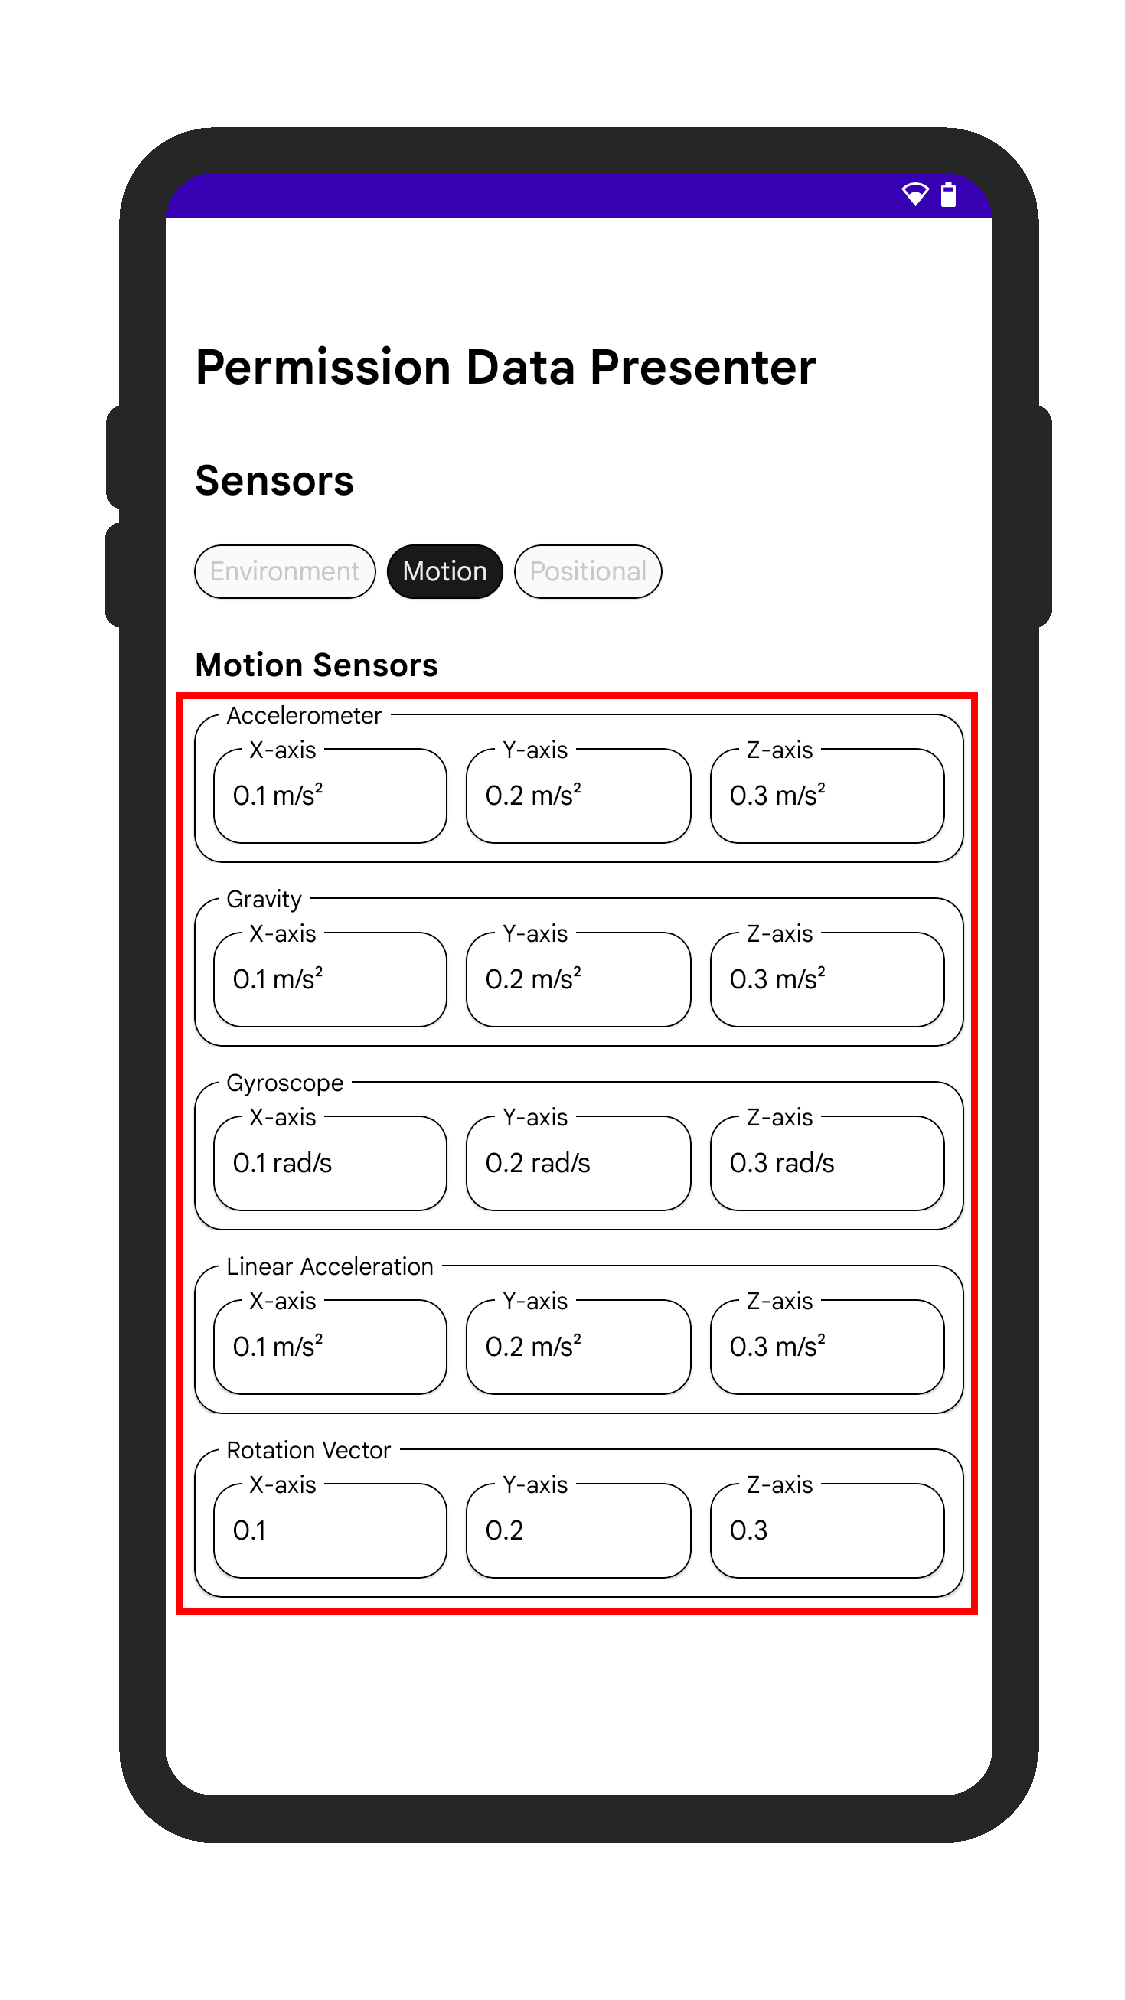
\includegraphics[width=\linewidth]{figures/case_studies/pdp_after_deceiving.pdf}
%    \caption{\centering With \framework{} (False sensor readings)}
%    \label{fig:case_study_pdp_w_frmwrk}
%\end{subfigure}
%\caption{\centering Screenshots of \textit{PDP} presenting readings of various motion sensors of the device by calling sensitive APIs}
%\label{fig:case_study_pdp}
%\end{figure}

%\framework{} effectively spoofed the diverse user data requested by PDP. This manipulation tricked PDP into believing that the received user data was accurate and subsequently transmitting it to the server. This serves as a stark reminder that users may struggle to protect the data stored on servers, but they can safeguard their privacy by controlling the amount of data shared with such servers.